\documentclass[conference]{IEEEtran}

\usepackage{amsmath, amsthm, amssymb, dsfont, accents}

\usepackage{tikz,pgfplots}
\usepackage{booktabs}
\usepackage[numbers]{natbib}
\usepackage{todonotes}
\definecolor{explore}{rgb}{0.8, 0.8, 1.0}
\definecolor{mission}{rgb}{0.59, 0.78, 0.64}

\pgfplotsset{compat=1.14}

\usetikzlibrary{calc, automata}
\newlength\figureheight
\newlength\figurewidth

\renewcommand{\cite}[1]{\citep{#1}}

\pdfinfo{
   /Author (Homer Simpson)
   /Title  (Robots: Our new overlords)
   /CreationDate (D:20101201120000)
   /Subject (Robots)
   /Keywords (Robots;Overlords)
}

% MDPs
\newcommand{\MDP}{\mathbb{M}}

\newcommand{\X}{\mathbb{X}}
\newcommand{\U}{\mathbb{U}}
\newcommand{\init}{\rho}
\newcommand{\tr}{T}

\newcommand{\pol}{\mu}

% LTL
\newcommand{\True}{\texttt{true}}
\newcommand{\False}{\texttt{false}}
\newcommand{\AP}{AP}

\newcommand{\ltluntil}{\mathcal{U}}
\newcommand{\ltlnext}{\bigcirc}

\newcommand{\alphabet}{{2^{\AP}}}
\newcommand{\word}{\boldsymbol{\pi}}
\newcommand{\letter}{\pi}
\newcommand{\lab}{L}

\newcommand{\FSA}{\mathcal{A}}

% Probability
\newcommand{\Prob}{\mathbf{P}}


% Value iteration
\newcommand{\bellman}{\mathcal{B}}


% Math
\DeclareMathOperator*{\argmin}{arg\,min}
\DeclareMathOperator*{\argmax}{arg\,max}
\newcommand{\ind}{\mathbf{1}}


\newtheorem{problem}{Problem}
\newtheorem{theorem}{Theorem}
\newtheorem{definition}{Definition}
\newtheorem{remark}{Remark}
\newtheorem{example}{Example}

\newcommand{\red}[1]{{\color{red} #1 }}
\newcommand{\sofie}[1]{{\color{orange}#1}}
\newcommand{\sofieNew}[1]{{\color{blue}#1}}
\begin{document}

%\title{\huge Sequential Value Iteration for Modular Systems Applied to Collaborative Space Robotics}

%\title{\huge Specification-oriented Active Exploration via Sequential Dynamic Programming: Applications to Space Exploration via a Rover-Copter Team}

%\title{\huge Specification-guided Active Exploration: Applications to Safety-critical Mars Rover-Copter Mission}

\title{\huge Specification-guided Active Exploration: Applications to a Risk-averse Rover/Copter Mars Mission}

%\title{\huge Verifiability-oriented Active Exploration: Applications to Safety-critical Mars Rover-Copter Team}

%\title{\huge Satisfaction-oriented Active Exploration: Applications to Safety-critical Mars Rover-Copter Team}

\author{Anonymous submission}

\maketitle

\begin{abstract}
  As a step towards achieving autonomy in space exploration missions we consider a collaborative robotics system with a copter and a rover. The goal of the copter is to explore an unknown environment so as to maximize knowledge about a science mission expressed in Linear Temporal Logic. We formulate the problem as a two-step stochastic dynamic program and mitigate the curse of dimensionality for this large system by leveraging its decomposed nature. We demonstrate in simulations that the robot team makes intelligent decisions in the face of uncertainty.
\end{abstract}

\IEEEpeerreviewmaketitle


%%%%%%%%%%%%%%%%%%%%%%%%%%%%%%%%%%%%%%%%%%%%%%%%
%%%%%%%%%%%%%%%%%%%%%%%%%%%%%%%%%%%%%%%%%%%%%%%%

\section{Introduction}

Environment exploration and task planning are crucial components of any autonomous system. In most approaches, these two aspects are decoupled in the sense that exploration is performed to maximize knowledge overall, rather than to maximize knowledge \emph{pertaining to the task}. In this work, we aim to improve efficiency in situations where exploration is expensive by limiting exploration to areas crucial for accomplishing a given task.

Due to the growing complexity and uncertainty in future space missions, autonomy is a crucial ability required for mission success. In this work, we focus on multi-asset missions (teams of robots), in particular the 2020 Mars mission that will consist of a ground rover and a copter for exploration (Fig. \ref{fig:heli-rover}). To increase productivity and science return, the robotic team needs to autonomously perform multi-sol (sol: martian day) navigation without human intervention. Severe communication delays and resource constraints (like battery time and limited hours of sunlight) pose further challenges in achieving such autonomy. In these missions, partial knowledge about the environment is typically available from satellite imagery, but it needs to be complemented with observations from on-board sensors. Our goal is to improve both autonomy and efficiency in such missions by developing principled methods that in a specification-guided manner determine the most important areas to explore. We focus specifically on the problem of determining how the copter should behave to assist the rover in the autonomous execution of mission tasks.

Our approach lies at the intersection of formal synthesis methods and stochastic optimal control; we phrase the exploration problem as a two-stage optimal control problem in the combined space of copter poses and environment beliefs. To partially circumvent the curse of dimensionality we leverage the decomposed nature of the problem and perform value iteration via sequential back-stepping, which avoids explicit construction of the large aggregate system.
\begin{figure}
  \begin{center}
    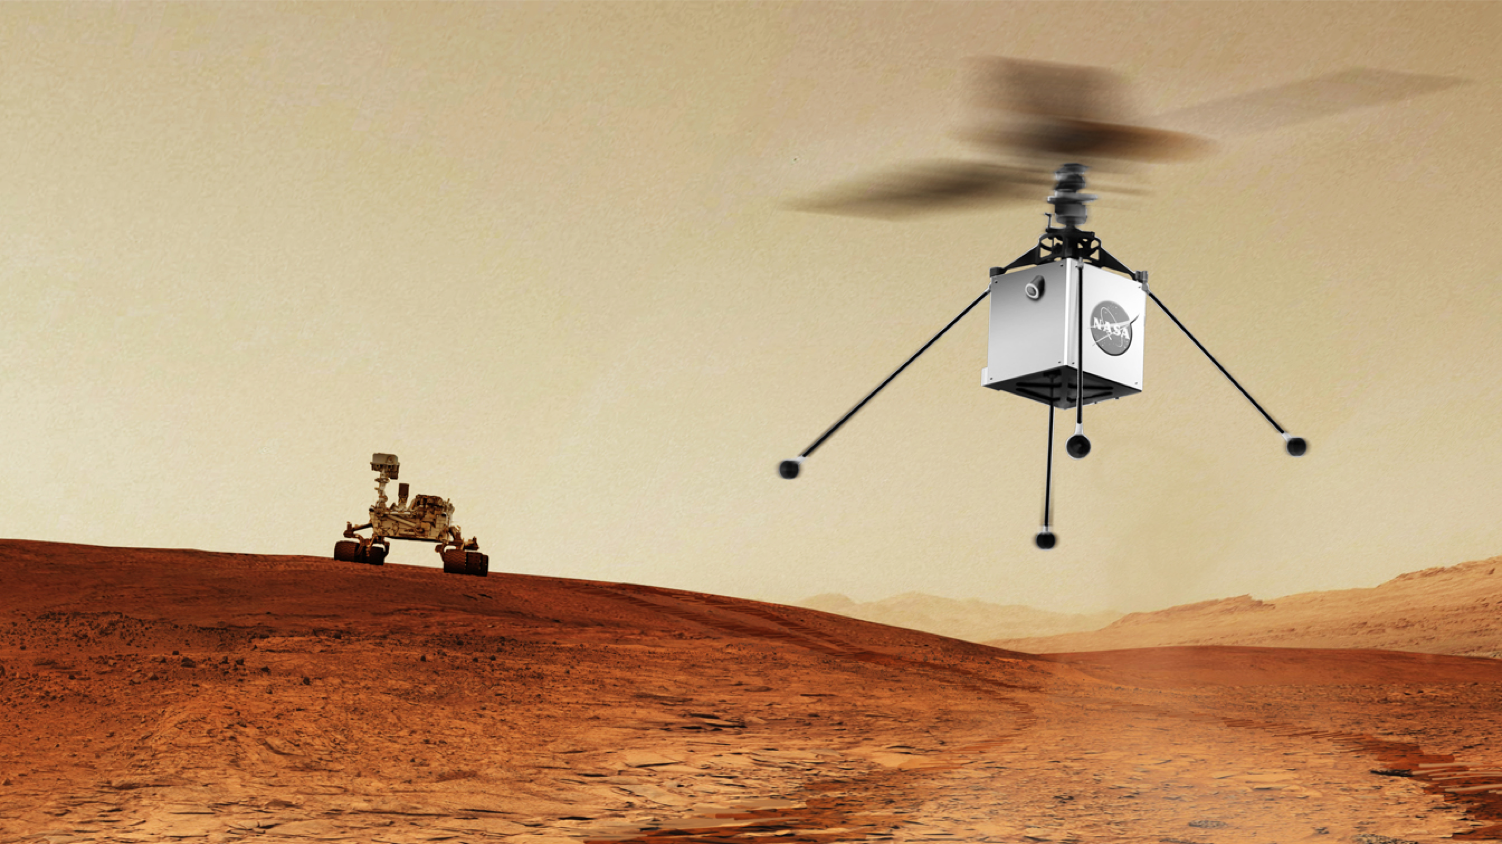
\includegraphics[width=0.8\columnwidth]{figs/heli-rover.png}
  \end{center}
  \caption{Cooperative robotics team for Mars exploration.}
  \label{fig:heli-rover}
\end{figure}

\subsection{Related work}
Environment mapping for robot navigational purposes is an important prerequisite for robotic autonomy for which many types of methods have been proposed \cite{Thrun2005,stachniss2009_book,thrun2002robotic}. While mapping algorithms can be developed separately from planning algorithms, in this work, we are interested in \emph{joint} planning and mapping methods. Active perception techniques fall into this category \cite{blake1992active, aloimonos1988active,soatto2013actionable}. Active mapping or SLAM algorithms, a subcategory of active perception, aims to enhance the quality of the environment map (e.g., for the navigation task \cite{Agha2017_ISRR,feder1999adaptive,davison2002simultaneous,Mu16-CDC}) by choosing information-rich trajectories. However, these methods are typically limited to subsystem autonomy (e.g., navigation) and do not have a principled way of incorporating system-level constraints and high-level mission specifications and requirements. In this work, we aim to develop a novel methodology that allows for principled incorporation of mission specifications where the ``active" perception not only helps navigation, but also assists with satisfaction of mission goals.

Three major classes of methods exist to solve stochastic optimal control problems: value iteration, policy iteration, and linear programming \cite{Bertsekas1978}. Approximate solutions methods to the stochastic optimal control problem under temporal logic constraints have been proposed via parametrized value function approximations \cite{Papusha2016,Leong2016}, and via tensor decompositions \cite{Alora2016}. While the above mentioned approaches are general in scope, we focus on uncertainty stemming from an unknown environment which we model in a way that leads to a naturally decomposed problem.


\subsection{Contributions and Paper Layout}

The contributions of this paper are threefold. Firstly, in Section \ref{sec:problem} we construct a novel problem formulation for future multi-asset Mars missions by modeling all systems components as Markov Decision Processes, and by expressing science objectives using temporal logics. Secondly in Section \ref{sec:stochopt}, we show that the exploration task can be reformulated as a stochastic optimal control problem that is specific to the task assigned to the rover. In the subsequent Section \ref{sec:valueiter} we introduce--as the third contribution--computational methods levering the inherent decomposed structure of the problem to mitigate the curse of dimensionality. Additionally in Section \ref{sec:casestudy}, we illustrate these new concepts on a case study that exhibits typical aspects of a Mars exploration problem, before concluding the paper in Section \ref{sec:conclusion}.


\section{Problem Setup}
\label{sec:problem}

\subsection{Markov Decision Process models}
We model the rover and copter as well as environment uncertainty as Markov Decision Processes. Consider the definition of a Markov Decision Process (MDP) as in \cite{Bertsekas1978}.
\begin{definition}
\label{def:MDP}
  A discrete-time \textbf{Markov decision process} (MDP) is a tuple $\MDP = (\X, x_0,\tr, \U)$ where
  \begin{itemize}
    \item $\X$ is a state space with states $x\in\X$; % as its elements;
    \item $x_0\in \X$ is the initial state;
    \item $\U$ is a input space with inputs $u\in\U$;
    \item $\tr$ is a conditional stochastic kernel that assigns to each state $x\in \X$ and control input $u\in \U$ a probability distribution $\tr(\cdot\mid x,u)$ over $\X$.
  \end{itemize}
\end{definition}
For a given sequence of control inputs $u_t \in \U$ with timing $t$, we say that an \emph{execution} of $\MDP$ initialized at $x_0$ is a sequence of states $\mathbf x = x_0x_1x_2x_3\ldots $ for which each state transition is obtained as a realization of the stochastic transition kernel $x_{t+1} \sim \tr(\cdot \mid x_t, u_t)$. A \emph{policy} $\pol = \pol_0 \pol_1 \ldots$ is a sequence of mappings $\pol_t:\prod_{t}\X\rightarrow \U$ from the history space to the action space. A controlled execution is generated by $\pol$ if each state transition is obtained as a realization of the stochastic transition kernel $x_{t+1} \sim \tr(\cdot\,{ \mid}\, x_t, \mu_t(x_0,\ldots,x_t))$.  A policy is \emph{Markov}  if for all $t$ it holds that  $\pol_t(x_0, \ldots, x_t) = \pol_t(x_t)$. All systems in this paper are modeled as MDPs, or as combinations (products) of MDPs.

\smallskip
\noindent{\bfseries Rover and copter as MDPs}.
In case of the rover the state space $\X$ represents the two-dimensional space in which the rovers navigates. Its state transitions can be modeled as being either stochastic or deterministic. Similarly, the dynamics of the copter can be represented in three-dimensional space, where the additional dimension represents altitude. Effects of wind and other uncertainty influencing the state transitions can be captured by the stochastic transitions in the copter MDP model. For brevity, we refer to this model as $\MDP_{cop}$ and index its state as $x^c$. Similarly, we refer to the rover model as an MDP $\MDP_{rov}$ with state $x^r$.

\smallskip
\noindent{\bfseries Environment uncertainty as a belief MDP.}
A common way to represent a map for planning purposes is to attach labels such as ``sand'' or ``rock'' to different \emph{regions}, but in a Mars setting the true labels are often only partially known at the time of system deployment.

We capture this environmental uncertainty with MDPs $\MDP_{e_i}$ that model belief dynamics over labeled regions $i$ of the two-dimensional rover state space. The aggregate environment model $\MDP_{env}$ with state $x^e$ is the combination of individual MDPs $\MDP_{e_i}$. Transitions in these MDPs occur when measurements are taken from on-board sensors, i.e., the stochastic kernels are parameterized by the physical distance of the robots to the regions in a measurement model. For instance, it is reasonable to assume that the rover can take measurements of a given region provided that it is sufficiently close, and that the copter can take measurements of regions it flies above. Copter measurements also depend on the altitude: a high-flying copter can see a larger area but the image resolution is better if the copter is close to the ground. Hence the measurement models dictate the structured composition of the copter and rover models with the environment model. The resulting composed MDP represents the full model of the state of both robots and the current knowledge of the environment.

\todo[inline]{Figure of copter and rover taking measurements of a region of interest}

\subsection{Formal specifications}
We use temporal logic formulas to formally describe tasks that the rover should perform. The basic building blocks of a temporal logic formula are \emph{atomic propositions} that take values $\True$ or $\False$.  An atomic proposition $p$ is associated with a subset $A$ of a state space $\X$ in the sense that $p = \True$ if and only if $x \in A$.

By combining atomic propositions into a formula, desired system behavior is expressed as set membership constraints (atomic propositions) together with temporal relations (operators). Consider a set $AP = \{ p_1, \ldots, p_L \}$ of atomic propositions; it defines an \emph{alphabet} $\alphabet$ where each \emph{letter} $\letter$ of the alphabet is defined as a set of atomic propositions. An infinite string of letters is a \emph{word} $\word=\letter_0\letter_1\letter_2\ldots$, which should be thought of as the observed output of a system. More specifically, for each execution $\mathbf{x} = x_0 x_1 x_2 \ldots$ of an MDP, a labeling function $\lab: \X \rightarrow \alphabet$ that maps states to outputs yields the associated word as $\word = \lab(x_0)\lab(x_1) \lab(x_2) \ldots$. Desired behavioral properties can now be expressed via temporal logic formulas over the generated words.

In the sequel we focus on a fragment of linear temporal logic.
\begin{definition}
  \label{def:gdtl-syntax}
  Formulas in the \textbf{syntactically co-safe LTL} (scLTL) fragment are constructed according to the grammar
  \begin{equation}
    \label{eq:scLTL}
    \varphi ::=  \True \, |\,p \, |\, \lnot p \, |\, \varphi_1 \vee\varphi_2  \, |\, \varphi_1 \land \varphi_2 \, |\, \varphi_1 \ltluntil \varphi_2 \, |\, \ltlnext \varphi,
  \end{equation}
  where $p\in \AP$ is an atomic proposition.
\end{definition}
The syntax defines the symbols and their correct ordering in a formula. In contrast, the semantics defined next give the interpretation of a formula.
\begin{definition}
 The \textbf{semantics} of scLTL are defined recursively as follows: $\word$ \textbf{satisfies} $\varphi$ at time $t$, written $(\word, t) \models \varphi$, if
 \begin{itemize}
    \item $(\word, t) \models \True$;
    \item $(\word, t) \models p$ iff $p \in \letter_t$;
    \item $(\word, t) \models \varphi_1 \land  \varphi_2  $ iff $ ( (\word, t) \models \varphi_1 ) \land ( (\word, t) \models \varphi_2 ) $;
    \item $(\word, t) \models \varphi_1 \lor  \varphi_2  $ iff $ ( (\word, t) \models \varphi_1 ) \lor ( (\word, t) \models \varphi_2 ) $;
    \item $(\word, t) \models  \varphi_1 \ltluntil \varphi_2 $ iff $\exists s \geq t \text{ s.t. } ((\word, s) \models \varphi_2 ) $ and $(\word, l) \models \varphi_1, \forall l \in \{t, \ldots s-1\}$;
    \item $(\word, t) \models \ltlnext \varphi$ iff $(\word, t+1) \models \varphi$.
 \end{itemize}

\end{definition}
We say that a state trajectory $\mathbf{x} = x_0 x_1 x_2 \ldots$ satisfies a specification $\varphi$, written $\mathbf{x} \models \varphi$, if the generated word $\word =\lab(x_0) \lab(x_1) \lab(x_2) \ldots$ satisfies $\varphi$ at time 0, i.e. $\letter_0 \models \varphi$.

In general, we cannot say that an MDP $\MDP$ satisfies a property $\varphi$ for a given policy $\mu$, since transitions are stochastic. However, we can quantify the probability that the system satisfies the property, i.e. compute or approximate
\begin{equation}
  \label{eq:probLTL}
  \mathbb P_{\mu}^\MDP[\mathbf x \vDash \varphi ].
\end{equation}

For our purposes, the interesting scenarios is when there is a lot of uncertainty about whether the mission can be completed or not. If the mission is trivial, or it is already known to be difficult, exploration will only further establish these facts. In cases where mission completion is uncertain, we want to leverage the copter to reduce \emph{mission risk}, defined as the probability that a mission we choose to undertake ultimately fails. Having introduced MDP models for rover, copter, and environment belief, as well as scLTL specifications, the problem we address in this paper can be stated as follows.

\begin{problem}
\label{prob:basic}
Consider a robot-copter team in an uncertain environment, all modeled as MDPs. Design a strategy for the robot-copter team that reduces the inherent risk of a scientific mission given as an scLTL formula.
\end{problem}

We have chosen to work with the scLTL fragment that is restricted to properties that can be satisfied in finite time. For the purpose of Mars exploration where tasks are often defined on a daily basis (and thus are of finite duration) this fragment is sufficient to express all relevant specifications.

\subsection{Problem Decomposition}

Due to the nature of the mission---the copter is quick and has short battery life (minutes), the rover moves slowly (over hours)---it is reasonable to divide the problem into two subproblems. 
% More specifically, we assume that the copter can complete its exploration before the rover enters the critical part of its scientific mission. 
We propose to solve the problem sequentially based on its natural division into two phases: exploration and mission execution. As shown in Fig. \ref{fig:execorder}, the copter is active in the exploration phase, whereas the rover conducts the critical scientific mission in the second phase. We assume that the exploration phase lasts for a time $T_c$, and that the mission phase lasts at most for a time $T_r$.
  %
%\begin{figure}
%	\begin{center}
%		\begin{tikzpicture}
%			\draw[|-|] (0,0) node[yshift=-1mm, anchor=north] {$0$} -- (3,0) node[yshift=-1mm, anchor=north] {$T_c$};
%			\draw[|-|] (3,0) -- (6,0) node[xshift=3mm, yshift=-1mm, anchor=north] {$T_c + T_r$};
%			\draw[|-latex] (6,0) -- (7,0) node[anchor=west] {$t$};
%
%			\node at (0,0.3) {$x_c$};
%			\node at (0,0.6) {$x_e$};
%
%			\node at (3,0.3) {$x_c$};
%			\node at (3,0.6) {$x_e$};
%			\node at (3,0.9) {$x_r$};
%
%			\node at (6,0.6) {$x_e$};
%			\node at (6,0.9) {$x_r$};
%
%			\draw[-latex] (0.5,0.3) -- (2.5,0.3);
%			\draw[-latex] (0.4,0.6) -- (2.5,0.6);
%
%			\draw[-latex] (3.5,0.9) -- (5.5,0.9);
%			\draw[-latex] (3.5,0.6) -- (5.5,0.6);
%
%			\node (expl) at (1.5, -0.5) {Exploration};
%			\node (miss) at (4.5, -0.5) {Mission};
%
%			\draw[dashed] (0,0) -- ($(expl.west)$);
%			\draw[dashed] (3,0) -- ($(expl.east)$);
%
%			\draw[dashed] (3,0) -- ($(miss.west)$);
%			\draw[dashed] (6,0) -- ($(miss.east)$);
%
%		\end{tikzpicture}
%	\end{center}
%	\caption{Illustration of execution order. In the exploration phase $[0, T_c]$ the copter explores the environment, whereas the rover executes the scientific mission on $[T_c, T_c + T_r]$.}
%	\label{fig:execorder}
%\end{figure}


\begin{figure}

\centering
	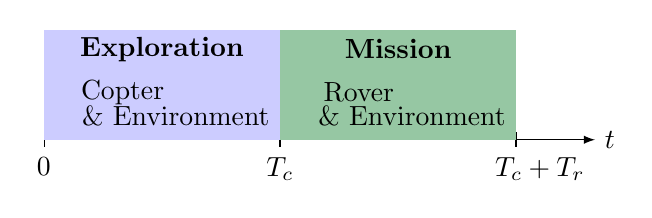
\begin{tikzpicture}
			\draw[|-|] (0,0) node[yshift=-1mm, anchor=north] {$0$} -- (3,0) node[yshift=-1mm, anchor=north] {$T_c$};
			\draw[|-|] (3,0) -- (6,0) node[xshift=3mm, yshift=-1mm, anchor=north] {$T_c + T_r$};
			\draw[|-latex] (6,0) -- (7,0) node[anchor=west] {$t$};
			\fill[color=explore]  (0,0) -- (3,0) -- (3,1.4) -- (0,1.4)--cycle;
				\fill[color=mission]  (3,0) -- (6,0) -- (6,1.4) -- (3,1.4)--cycle;

%			\node at (0,0.3) {$x_c$};
%			\node at (0,0.6) {$x_e$};
			\node at (1.5,0.3) {\ \ \ \& Environment};
			\node at (4.5,0.3) {\ \ \ \& Environment};
			\node at (1,0.6) {Copter};
			\node at (4,0.6) {Rover};
%			\node at (3,0.3) {$x_c$};
%			\node at (3,0.6) {$x_e$};
%			\node at (3,0.9) {$x_r$};
%
%			\node at (6,0.6) {$x_e$};
%			\node at (6,0.9) {$x_r$};

%			\draw[-latex] (0.5,0.3) -- (2.5,0.3);
%			\draw[-latex] (0.4,0.6) -- (2.5,0.6);
%
%			\draw[-latex] (3.5,0.9) -- (5.5,0.9);
%			\draw[-latex] (3.5,0.6) -- (5.5,0.6);


			\node (expl) at (1.5, 1.15) {\bfseries \color{black} Exploration};
			\node (miss) at (4.5, 1.15) {\bfseries \color{black} Mission};

%			\draw[dashed] (0,0) -- ($(expl.west)$);
%			\draw[dashed] (3,0) -- ($(expl.east)$);
%
%			\draw[dashed] (3,0) -- ($(miss.west)$);
%			\draw[dashed] (6,0) -- ($(miss.east)$);

		\end{tikzpicture}
			\caption{Illustration of execution order. In the exploration phase $[0, T_c]$ the copter explores the environment, whereas the rover executes the scientific mission on $[T_c, T_c + T_r]$.}	\label{fig:execorder}
\end{figure}
%
%We consider a system consisting of the following components:
%\begin{enumerate}
%	\item An MDP $\MDP_{rov}$ with state $x_r$ modeling a ground rover in 2D space.
%	\item An MDP $\MDP_{env}$ with state $x_e$ that captures belief dynamics over a collection of unknown environment labels.
%	\item A scLTL specification $\varphi$ that expresses the requirement of the scientific mission. The formula is defined over a set of atomic propositions in $\X_{rov} \times \X_{env}$---the combined space of rover poses and environment beliefs.
%	\item An MDP $\MDP_{copt}$ modeling a copter in 3D space.
%	\item A measurement model that dictates how the state of $\MDP_{env}$ is updated from measurements received from the rover and copter. For instance, it is reasonable to assume that the rover can take measurements of a given region provided that it is sufficiently close, and that the copter can take measurements of regions it flies above. Copter measurements also depend on the altitude: a high-flying copter can see a larger area but the image resolution is better if the copter is close to the ground.
%\end{enumerate}
These times can be determined based on the available battery capacity and remaining hours of daylight. In both phases the environment belief is updated according to measurements taken by the active agent. While the execution order of the phases is exploration first and the mission execution, the reverse holds for design: first the mission design problem is solved and its solution informs the exploration design.

\smallskip
\noindent{\bfseries Mission Problem:} The objective in the mission phase is to maximize the probability that the specification $\varphi$ is satisfied, thus part of the Mission Problem is to synthesize such a policy. However, to guide the design of an exploration policy it is also necessary to quantify the probability of success for different environment belief states at time $T_c$. To this end, the objective of the Mission Problem is to for a given initial rover state $x^r_{0}$, for all environment belief states $x^e_{T_c}$ compute the probability that the mission specification is satisfied, along with a maximizing policy.
% \begin{equation}
 	% R(x^e_{T_c}) = \max_{\mu_1}\mathbb P_{\mu_1}^\MDP[\mathbf x \vDash \varphi \mid x^r_0, x^e_{T_c} ],
% \end{equation}
% along with a policy $\mu_1$ that maximizes the probability of specification satisfaction.

\smallskip
\noindent{\bfseries Exploration Problem:} Our objective is to extract control policies that maximize the knowledge about the satisfiability of a given task: either we want the exploration to show that the task can be completed with a high probability, or that the probability of task completion is very low. Both are desirable outcomes since a negative results allows resources to be redirected towards more realistic objectives. Based on the partition into exploration and mission phases we refine our problem as follows.
\begin{problem}
\label{prob:main}
  Consider the model components listed above. Design a policy for the copter exploration phase that explores the environment in a way that maximizes the expected knowledge about satisfaction of the scientific mission at time $T_c$.
\end{problem}

\smallskip
\noindent{\bfseries Computational Challenge:} Due to the multiple interacting model components, a solution to Problem \ref{prob:main} is potentially computationally challenging. The decomposition into an exploration phase and a mission phase already improves scalability significantly by limiting the number of systems that are active at any given time (c.f. Fig. \ref{fig:execorder}). We additionally show in Section \ref{sec:valueiter} how the problem can be solved sequentially over system components, which avoids the expensive step of explicit computation of transition probabilities in the aggregate systems. Combined, these two innovations allow us to synthesize policies for realistic problems of modest size.


\section{A Stochastic Optimal Control Approach}
\label{sec:stochopt}

% We now show that both subproblems can be solved as stochastic optimal control problems characterized by a Bellman operator
% %Given a function $g: \X \times \mathbb{R}_+ \rightarrow \mathbb{R}_+$, consider a general Bellman operator
% %$\bellman : (\X \rightarrow \mathbb{R}_+) \rightarrow (\X \rightarrow \mathbb{R}_+)$ on the following form:
% \begin{equation}
%   (\bellman V) (x) =  \max_{u \in \U}\mathbb E \left[ g(x', V(x')) \right]  \mbox{ for } x'\sim  T(\cdot \mid x, u).
% \end{equation}
% where $g:\X \times \mathbb{R}_+ \rightarrow \mathbb{R}_+$ is a problem-specific function and the value functions $V:\X\rightarrow \mathbb{R}_+$ are positive definite mappings defined on state space $\X$.

The exploration phase impacts the execution of the mission phase via the shared knowledge of the environment. Since we are interested in solving the exploration in such a way that the impact on the rover mission is maximized, we first characterize the probability of rover mission success as a function of the environment belief. We then leverage this knowledge to design an exploration optimal control problem.


\subsection{Mission-Phase Optimal Control}
We first show that specification satisfaction is related to a stochastic reachability problem over an extended MDP, and then detail how it can be written as a stochastic finite-horizon dynamic programming problem. We start with an example illustrating how product systems can be used to reason about specification satisfaction.

\begin{example}
\label{example:automaton}
Consider the example in Fig. \ref{fig:specautomaton} consisting of an example MDP and a mission specification $\varphi = \lozenge a \wedge \lozenge b$ dictating that two tasks $a$ and $b$ should both eventually be satisfied. The atomic proposition $a$ is associated with state $x^a$ whereas $b$ is associated with $x^b$, i.e. the labeling function is $L(x^a) = \{ a \}$, $L(x^b) = \{b \}$ and $L(x^c) =\emptyset$. We can construct the system to the right in Fig. \ref{fig:specautomaton} that has the property that a trace $\mathbf \pi=L(x_0) L(x_1) L(x_2)\ldots$ satisfies the specification if and only if the sequence of control inputs $\pi$ to this system reaches the target state $q_f$. All trajectories reaching $q_f$ have the property that both $a$ and $b$ have been observed, and all trajectories with this property reach $q_f$.

\begin{figure}[htp]
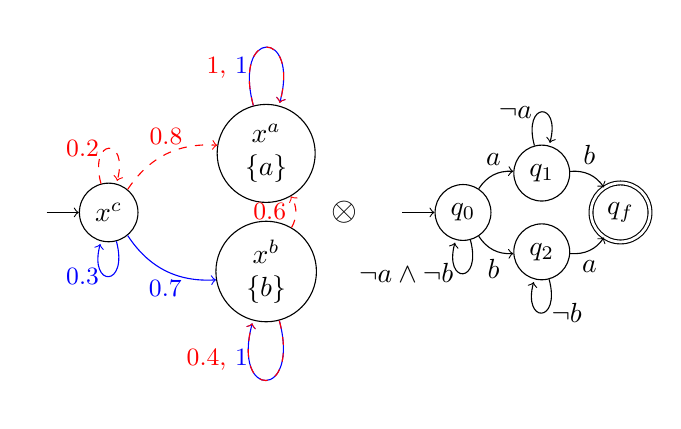
\begin{tikzpicture}[node distance =2cm,scale=0.9]
      \node[initial,  initial text={},name = init,circle,draw] {$x^c$};
    \node[circle, draw,right of = init, yshift = .75cm,align=center] (x1){$x^a$ \\ $\{a\}$ };
    \node[circle, draw, right of = init, yshift = -.75cm, align=center](x2) {$x^b$ \\ $\{b\}$};
    \path[->] (init) edge [bend left, dashed, red]
 node[above] {\small $ 0.8$} (x1)
 (init) edge [loop above, dashed, red]
 node[left] {\small$0.2$} (init)
 (init) edge [bend right, blue]
 node[below] {\small$ 0.7$} (x2)
  (init) edge [loop below, blue]
 node[left] {\small$0.3$} (init)
 (x2) edge [bend right,dashed, red]
 node[left] {\small$0.6$} (x1)
  (x2) edge [loop below, blue](x2)
   (x2) edge [loop below,dashed, red]
 node[ above left] {\small \textcolor{red}{0.4}, \textcolor{blue}{1}\ \ } (x2)
  (x1) edge [loop above, blue](x1)
   (x1) edge [loop above,dashed, red]
 node[ below left ] {\small \textcolor{red}{1}, \textcolor{blue}{1}\ \ } (x1) ;
 \node[right of= x2, yshift = .75cm, node distance = 1cm, name=prod]{\large$\otimes$};

 %		\path[->] (init) edge [bend left] node[above] {$a$} (A)
%		(init) edge [bend right] node[below] {$b$} (B)
%		(init) edge [loop below] node[left] {$\neg a \wedge \neg b$} (init)
%		(A) edge [loop above] node[left] {$\neg a$} (A)
%		(B) edge [loop below] node[right] {$\neg b $} (B)
%		(B) edge [bend right] node[below] {$u_1$} (AB)
%		(A) edge [bend left] node[above] {$u_1$} (AB);
		\node[initial, right of = prod,initial text={},name = init,circle,draw, node distance=1.5cm] {$q_0$};
		\begin{scope}[node distance =1cm]
			\node[circle, draw,right of = init, yshift = .5cm] (A){$q_1$};
		\node[circle, draw, right of = init, yshift = -.5cm](B) {$q_2$};
		\node[ circle, draw,right of = B, yshift = .5cm, double, double distance=1pt] (AB){$q_f$};
		\path[->] (init) edge [bend left] node[above] {$a$} (A)
		(init) edge [bend right] node[below] {$b$} (B)
		(init) edge [loop below] node[left] {$\neg a \wedge \neg b$} (init)
		(A) edge [loop above] node[left] {$\neg a$} (A)
		(B) edge [loop below] node[right] {$\neg b $} (B)
		(B) edge [bend right] node[below] {$a$} (AB)
		(A) edge [bend left] node[above] {$b$} (AB);
		\end{scope}

	\end{tikzpicture}
	\caption{On the left an example MDP, and on the right a finite state system associated to mission specification $\varphi:= \lozenge a \wedge \lozenge b$.  }
  \label{fig:specautomaton}
\end{figure}
\end{example}

The procedure in Example \ref{example:automaton} is general: for any specification $\varphi$ in the scLTL fragment it is possible to construct a finite-state automaton $\FSA_\varphi$ with accepting set $Q_f$ \cite{Belta2017}. A finite-state automaton is a special case of an MDP. Thus, the probability \eqref{eq:probLTL} that a specification is satisfied for an MDP $\MDP$ with state space $\X$ is equivalent to the probability that a set $\X\times Q_f$ in the state space of the extended product system $\MDP \otimes_{ser}^L \FSA_\psi$ is reached, where the product $\otimes_{ser}^L$ is defined as follows:
\begin{definition} Consider two MDPs  $\MDP_1$ and $\MDP_2$. For a given \textbf{connection} $C : \X_1 \rightarrow \U_2$, their \textbf{serial product} is the MDP $\MDP_1 \otimes_{ser}^C \MDP_2 = (\X_1 \times \X_2, x_{ser}, \U_1, \tr_{ser})$, for $x_{ser}:= (x_{1,0},x_{2,0})$
  with %$\init_{ser}= \init_1(x_1) \init_2(x_2)$
 % and
  \begin{equation}\label{eq:serial}
  \begin{aligned}
      \tr_{ser}&(x_1', x_2' \mid x_1, x_2, u_1) \\
      & = \tr_1 (x_1' \mid x_1, u_1) \tr_2 (x_2' \mid x_2, C(x_1') ).
  \end{aligned}
  \end{equation}
  Additionally, we say that their  \textbf{parallel product} is the MDP $\MDP_1 \otimes_{par} \MDP_2 = (\X_1 \times \X_2, x_{par}, \U_1 \times \U_2, \tr_{par})$,  for $x_{par}:= (x_{1,0},x_{2,0})$ with
%where $\init_{par}(x_1, x_2) = \init_1(x_1) \init_2(x_2)$  and
  \begin{equation}
  \begin{aligned}
      \tr_{par}&(x_1', x_2' \mid x_1, x_2, u_1, u_2) \\
      & = \tr_1 (x_1' \mid x_1, u_1) \tr_2 (x_2' \mid x_2, u_2).
  \end{aligned}
  \end{equation}
\end{definition}

 Let us now look at the specific case of the rover mission. The MDP model of this mission contains both the rover $\MDP_{rov}$ and environment $\MDP_{env}$.
Since   the environment belief MDP itself is composed of several belief MDPs over individual labels, i.e., $\MDP_{env}:=\left( \MDP_{e_1} \otimes_{par} \ldots \otimes_{par} \MDP_{e_n} \right) $, it follows that the mission MDP is given as
\begin{equation}
  \left( \MDP_{rov} \otimes_{ser}^{C_1}\left( \MDP_{e_1} \otimes_{par} \ldots \otimes_{par} \MDP_{e_n} \right) \right)
\end{equation}
where $C_1 : \X_{rov} \rightarrow \U_{e_1} \times \ldots \times \U_{e_n}$ is a measurement model that maps rover poses to measurements in the environment model.

Moreover, when combined with the temporal specification $\varphi$ we get an extended MDP composed of different parts: the rover, the environment belief model, and also the specification automaton.
 \begin{equation}
\label{eq:syst_prod_def}
	\MDP_1 = \left( \MDP_{rov} \otimes_{ser}^{C_1} \left( \MDP_{e_1} \otimes_{par} \ldots \otimes_{par} \MDP_{e_n} \right) \right) \otimes_{ser}^{L} \mathcal A_{\varphi}.
\end{equation}
Here $L : \X_{rov} \otimes \X_{env} \rightarrow \U_{\varphi}$ maps the joint space of rover poses and environment belief states to $2^{AP}$, where $AP$ is the set of atomic propositions used to construct $\varphi$. To design a policy for the mission, it is now sufficient to maximize the probability that the extended MDP \eqref{eq:syst_prod_def} reaches the target set $\X_{rov} \otimes \X_{env} \otimes Q_f$.

Recall that the rover performs the mission task from time instant $T_c$ (the end time of the copter exploration) until time $T_r + T_c$. Thus for a given  policy $\mu$ the probability of mission specification satisfaction \eqref{eq:probLTL} can be expressed as
\begin{equation}
\begin{aligned}
\mathbb{P}_\mu \left[ \mathbf{x}_{[T_c,T_c+T_r]} \models \varphi \right].
\end{aligned}
\end{equation}
where $\mathbf{x}_{[T_c,T_c+T_r]}$ is the state trajectory over the interval $[T_c,T_c+T_r]$ of the rover and environment.
By incorporating the specification as part of the model, we can write an equivalent design problem as follows: %  can now be rewritten as
\begin{equation}
  \label{eq:ev_target}
  \argmax_{\mu_1} \mathbb{P}_{\mu_1}^{\MDP_1} \left[ \mathbf{x}_{[T_c,T_c+T_r]}^1 \models \lozenge X_f \right]
\end{equation}
with  $\mathbf{x}_{[T_c,T_c+T_r]}^1$ being the state trajectory of the extended MDP $\MDP_1$ and with the target set $X_f=\X_{rov} \otimes \X_{env} \otimes Q_f$.

% Given an indicator function $\mathbf 1_{X_f}:\X_1\rightarrow\{0,1\}$ with  $\mathbf 1_{X_f}(x) = 1 $ if $x\in X_f$ and $\mathbf 1_{X_f}(x) = 0$ otherwise, the probability \eqref{eq:ev_target} is equal to \(\mathbb{P}_{\mu} \left[\max_{x\in \mathbf{x}^{[T_c,T_c+T_r]}} \mathbf 1_{X_f}(x) \right]\)
% and for a given set of policies $\Pi$, the design problem is equal to
% \begin{equation}
%   \label{eq:optmission}
%   \max_{\mu\in \Pi}\mathbb{P}_{\mu}^{\MDP_1} \left[\max_{x\in \mathbf{x}^{[T_c,T_c+T_r]}} \mathbf 1_{X_f}(x) \right]
% \end{equation}
% Remark that we only need to consider the mission design $\mu=\mu_{T_c}\mu_{T_c+1}\ldots \mu_{T_c+T_r}$ for which each policy instance only controls the rover, that is, $\mu_{t}:\X_{rov}\times\X_{env}\times\X_\varphi\rightarrow \U_{rov}$.

To solve the optimal reachability problem \eqref{eq:ev_target}, we define a value function $V_r$ that quantifies the probability that the rover satisfies its specification before time $T_r + T_c$ as a function of the system state $x_{t}:=(x_{t}^r, x_{t}^e, x_{t}^\varphi)$ of $\MDP_1$ at time $t\geq T_c$:
\begin{equation}
\label{eq:rovervalue}
\begin{aligned}
	& V_r(x_{t}^r, x_{t}^e, x_{t}^\varphi)  = \max_{\mu_1} \mathbb{P}_{\mu_1}^{\MDP_1} \left[\mathbf{x}^1_{[t,T_c+T_r]} \models \lozenge X_f \mid \mathbf{x}_{[t]}^1 = x_{t} \right].
\end{aligned}
\end{equation}
Starting from $ V^{T_c+T_r}(x)\equiv \ind_{X_f}(x)$, this probability can be inductively computed, via \emph{value iterations}, along with the optimal, Markov policy as
  \begin{align}
    & V^{t}(x)  = \max_{u \in \U_{rov}}  \max( \ind_{X_f}(x), \mathbb{E}\left[V^{t+1}(x_{t+1}){\mid} x_t,u\right] )\label{eq:value_iter_mission}, \\
    & \pol_1^t(x) \in \argmax_{u\in \U_{rov}} \left(\max( \ind_{X_f}(x), \mathbb{E}\left[V^{t+1}(x_{t+1}){\mid }x_t,u\right] ) \right)\notag%\mathbb E \left[ \max( \ind_{X_f}(x'), V^{t+1}(x')) \right] .
    \end{align} 
for $x_{t+1}\sim  T(\cdot\,{ \mid}\, x_t, u)$, and with $\ind_{X_f}$ is the indicator function. 
%
We now have a full characterization of the value iteration and policy computation similar to  \cite{Abate2008}. 
Furthermore, for every Markov policy $\mu_1$ for the extended MDP $\MDP$ there exists a policy $\mu$ for the rover-mission MDP.
But the nested products in e.g. \eqref{eq:syst_prod_def} lead to large aggregate state spaces, and since the size of the transition matrix is quadratic in the size of the state space, computation of the aggregate transition matrix quickly becomes challenging. In the next section we show that value iteration can be done sequentially over subsystems without computing aggregate transition matrices, but first we discuss the exploration problem.

\subsection{Exploration Problem: Task-Specific Information Gathering}
\label{sub:information}

Similarly to above, we can model the overall stochastic system that is active in the exploration phase as
\begin{equation}
\begin{aligned}
	\MDP_2 & = \MDP_{cop} \otimes_{ser}^{C_3} \left( \MDP_{e_1} \otimes_{par} \ldots \otimes_{par} \MDP_{e_n} \right),
\end{aligned}
\end{equation}
with $C_3 : \X_{cop} \rightarrow \U_{e_1} \times \ldots \times \U_{e_n}$ being a measurement model that maps copter poses to measurements of the environment labels.
The exploration phase affects the environment belief $x^e$ at time $T_c$. We quantify the effect of the exploration as \emph{mission risk} $R:\X_{env}\rightarrow [0,1]$ defined as
\begin{equation}
	R(\cdot) = V_r(x_{T_c}^r, \cdot, x_{T_c}^\varphi),
\end{equation}
as a function of the environment belief state $x^e_{T_c}$, at the end of the exploration phase. Given $V_r(x_{T_c}^r, \cdot, x_{T_c}^\varphi)$, the question becomes how the environment should be explored in order to maximize knowledge (i.e. maximize the probability of a favorable $x^{e}_{T_c}$)?

We now question what a good result would be. As a first consideration, one could choose the exploration objective
\begin{equation}
\label{eq:badmeasure}
	\max_{\mu_{2}}\  \mathbb E^{\mathbb M_{2}}_{\mu_2} (R(x_{T_c}^e) )
\end{equation}
which simply attempts to maximize the probability that the rover can satisfy the mission specification. We give a small example, distilled from the larger Mars mission, that highlights issues with this objective.

\begin{example}[]
	Consider an environment with a single belief state $x^e\in[0,1]$ that expresses the belief that region $A$ contains a sample of interest.
	We specify the science mission as ``\emph{get  sample of $A$}'', i.e.,  $\lozenge A_s$, which is satisfied when $A$ is reached and $A$ contains a sample.
	Without loss of generality, assume that the rover can reach $A$ with probability 1 for a policy $\mu_R$. Then $\mu_R$ is an optimal policy for the rover and the satisfaction probability is equal to the initial belief state $x^e_{0}$.

  Even if the copter can explore region $A$ and thus determine exactly whether the mission can succeed or not, there is no benefit in doing so under the objective \eqref{eq:badmeasure}. Exploring $A$ has an expected utility of $\mathbb{E} \left[ x_{T_c}^e \right] = 1\times x^e_{0} +  0\times (1- x^e_{0}) = x^e_0$, i.e. identical to the initial value of \eqref{eq:badmeasure}.
\end{example}

Rather than naively maximizing the probability of satisfaction which can discourage exploration, we also consider it a positive outcome if the exploration phase shows that the probability of satisfying the mission is very low. Based on such knowledge resources can be redirected to more promising missions. We can separate possible outcomes of the exploration phase into:

\begin{enumerate}
	\item High confidence in mission satisfaction, i.e.,
\begin{equation}\label{eq:accept}
	R(x^e_{T_c})\geq 1-\delta_{acc}
\end{equation}
where $\delta_{acc}$ is the acceptable mission risk and the mission can be accepted,
	\item Very low confidence in mission satisfaction,  i.e.,
\begin{equation}\label{eq:reject}
	R(x^e_{T_c})\leq \delta_{rej},
\end{equation}
where $\delta_{rej}$ is the acceptable rejection risk for which the  rover mission can be aborted,
	\item Neither low nor high confidence in the mission satisfaction,
	 \begin{equation}
	\delta_{rej} \leq R(x^e_{T_c})\leq 1-\delta_{acc}.
\end{equation}
\end{enumerate}
The third outcome is the least useful for decision-making purposes as it is associated with the most uncertainty about task feasibility.

Based on this classification we consider the mission exploration a success if it results in $x_e^{T_c}$ being either in the acceptable region or in the abort region. Additionally, by the end of the exploration the copter should land  in region $x^{T_c}_c$. We can define this target region in the copter - environment space as
\begin{equation}
Y_\delta = \{x_{T_c}^c\}\times
	\{x^e_{T_c} \mbox{ s.t.  }\eqref{eq:accept}\mbox{ or s.t. }\eqref{eq:reject} \}.
\end{equation}
And we can specify the objective of the copter as
\begin{equation}
\label{eq:coptervalue}
	V^0_c(x^c_0, x^e_0) = \max_{\mu_2} \mathbb{P}_{\mu_2}^{\MDP_2} \left[ \mathbf{x}^2_{[0, T_c]} \models \lozenge Y_\delta \mid \mathbf{x}_{[0]} = (x^c_0, x^e_0) \right].
\end{equation}
where we have used the symbol $Y_\delta$ as an atomic proposition for the associated set.
Again this value and the associated optimal policy can be computed with value iterations \eqref{eq:value_iter_mission}.


In conclusion, in this section we have derived the following. For given initial poses $x^c_0$ and $x^r_0$ of the copter and robot, and an initial environment belief $x^e_0$, the function $V^0_c(x^c_0, x^e_0)$ as computed above is the probability that the exploration phase results in the task $\varphi$ being satisfiable with either probability at least $1- \delta_{acc}$, or with probability at most $\delta_{rej}$.
\subsection{Related work}
\sofieNew{The proposed design methodology depends on the utility for decision making as described in \cite{lindley2000philosophy}.  A similar formulation has been proposed in \cite{haesaert2016experiment} for the design of experiments.}

\section{ Value Iteration for Product MDPs}
\label{sec:valueiter}

As detailed in the previous section, the aggregate systems $\MDP_1$ and $\MDP_2$ for the mission and exploration phases are both formed as MDP products. Explicit construction of these aggregate systems quickly becomes computationally challenging. In this section we show that explicit construction is not required for certain types of value iteration---it can be performed recursively over the product components.

Given a function $g: \X \times \mathbb{R}_+ \rightarrow \mathbb{R}_+$, consider a general Bellman operator\footnote{\sofieNew{Remark that for this set of Bellman recursions, the control input is not rewarded directly, it only influences the value function via its effect on the next state distribution.}} $\bellman$ on the following form:
\begin{equation}
(\bellman V) (x) =  \max_{u \in \U} g \left( x, \mathbb E \left[  V(x') \mid x,u \right] \right).
\end{equation}
where $g$ is a problem-specific function and the value functions $V:\X\rightarrow \mathbb{R}_+$ are positive definite mappings defined on state space $\X$. For example, $g(x, v') = \max(\ind_{X_f}(x), v')$ corresponds to the Bellman operator for reachability of a set $X_f$ that we used in Section \ref{sec:valueiter}. Finite-horizon value iteration over a horizon $[0, T]$ consists of the following iterations:
\begin{equation}
\begin{aligned}
	V_T(x) & = g(x, 0), \quad V_{t-1} = \bellman V_t,\\
	\mu_t(x) & \in \argmax_{u \in \U} g(x, \mathbb{E}\left[ V(x') \mid x,u \right])
\end{aligned}
\end{equation}

We now consider the Bellman iteration step for product MDPs. For a serial product $\MDP = \MDP_1 \otimes_{ser}^{C} \MDP_2$ we get
\begin{equation*}
\begin{aligned}
	&  \mathbb{E}^\MDP\left[ V(x_1', x_2') \mid x_1, x_2, u_1 \right] \\ 
	& = \mathbb{E}^{\MDP_1} \left[ \mathbb{E}^{\MDP_2} \left[ V(x_1', x_2') \mid x_2, C(x_1')  \right] \mid x_1, u_1   \right],
\end{aligned}
\end{equation*}
where we note that the inner expectation is a function of $x_2$ and $x_1'$.
% \begin{equation*}
% \begin{aligned}
%   & \bellman V (x_1, x_2) = \max_{u_1 \in \U_1} \hspace{-2mm} \sum_{x_1', x_2' \in \X_1 \times \X_2}  \left[ \begin{aligned}
%   	g(x_1', x_2', V(x_1', x_2')) \\
%   	\times T_{ser}(x_1', x_2' \mid x_1, x_2, u_1)
%   \end{aligned} \right] \\
%   & = \max_{u_1 \in \U_1} \sum_{x_1' \in \X_1}  T_1(x_1' \mid x_1, u_1 ) \left[ \begin{aligned}
%    	\sum_{x_2' \in \X_2}  g(x_1', x_2', V(x_1', x_2')) \\
%    	\times  T_2(x_2' \mid x_2, C(x_1'))
%    \end{aligned} \right].
% \end{aligned}
% \end{equation*}
It follows that the Bellman update $V \mapsto \bellman V$ for a serial product can be computed in back-stepping fashion as follows:
\begin{equation*}
\begin{aligned}
	W_2(x_1', x_2) & = \mathbb{E}^{\MDP_2} \left[ V(x_1', x_2') \mid x_2, C(x_1')  \right], \\
	W_1(u_1, x_1, x_2) & = \mathbb{E}^{\MDP_1} \left[ W_2(x_1', x_2) \mid x_1, u_1   \right], \\
	\bellman V(x_1, x_2) & = \max_{u_1 \in \U_1} g(x_1, x_2, W_1(u_1, x_1, x_2)).
\end{aligned}
\end{equation*}
% \begin{equation*}
% \begin{aligned}
%   W_2(x_1', x_2') & = g(x_1', x_2', V(x_1', x_2')) \\
%   W_1(x_1', x_2) & = \sum_{x_2' \in \X_2}  T_2(x_2' \mid x_2, C(x_1')) W_2(x_1', x_2'), \\
%   \bellman V(x_1, x_2) & = \max_{u_1 \in \U_1} \sum_{x_1' \in \X_1} T_1(x_1' \mid x_1, u_1) W_1(x_1', x_2).
% \end{aligned}
% \end{equation*}
The procedure generalizes immediately to $n$-length serial products where the $(n-i)$th step becomes
\begin{equation}
\label{eq:general_decomp}
\begin{aligned}
	& W_i (\ldots, x_{i-1}', x_i, x_{i+1} \ldots) \\
	& = \mathbb{E}^{\MDP_i}\hspace{-0.5mm}  \left[ W_{i+1} (\ldots, x_{i-1}', x_i', x_{i+1} \ldots) \hspace{-0.5mm} \mid\hspace{-0.5mm}  x_i, C_i(x_{i-1}') \right].
\end{aligned}
\end{equation}
% \begin{equation}
% \label{eq:general_decomp}
% \begin{aligned}
%   & W_{i-1}(x_1', \ldots, x_{i-1}', x_i, \ldots, x_n) \\
%   & \quad = \sum_{x_{i}' \in \X_{i}} \left[ \begin{aligned} & T_{i} (x_{i}' \mid x_{i}, C(x_{i-1}')) \\ 
%    & \times W_{i} (x_1', \ldots, x_{i-1}', x_i', \ldots, x_n)
%     \end{aligned} \right].
% \end{aligned}
% \end{equation}

\begin{remark}
  In serial products of arbitrary length a connection $C_i$ can be defined either as $C_i: \X_{i-1} \rightarrow \U_i$, or as $C_i: \prod_{j \in \Gamma_i} \X_j \rightarrow \U_i$ for some index set $\Gamma_i$ that determines which preceding systems that affect the input to system $i$.
\end{remark}

In addition, if $\MDP_{i}$ is itself a serial or parallel product, the computation \eqref{eq:general_decomp} can again be performed via recursive back-stepping. If for instance $\MDP_{i} = \MDP_{i_1} \otimes_{par} \MDP_{i_2}$ is a parallel product we can write $x_i = (x_{i_1}, x_{i_2})$ and \eqref{eq:general_decomp} can be computed as
\begin{equation}
\begin{aligned}
	& W_{i_1}(\ldots (x_{i_1}', x_{i_2}) \ldots) \\
	& \quad = \mathbb{E}^{\MDP_{i_2}} \left[ W_{i+1}(\ldots (x_{i_1}', x_{i_2}') \ldots) \mid x_{i_2}, C_i(x_{i-1}) \right], \\
	& W_{i}(\ldots (x_{i_1}, x_{i_2}) \ldots) \\
	& \quad = \mathbb{E}^{\MDP_{i_1}} \left[ W_{i_1}(\ldots (x_{i_1}', x_{i_2}) \ldots) \mid x_{i_1}, C_i(x_{i-1}) \right].
\end{aligned}
\end{equation}
% \begin{equation*}
% \begin{aligned}
%   W_{i_1}(\ldots (x_{i_1}', x_{i_2}) \ldots) & = \hspace{-2mm} \sum_{x_{i_2}'  \in \X_{i_2}} \left[ \begin{aligned} T_{i_2}(x_{i_2}' \mid x_{i_2}, C(x_{i-1}') ) \\ \times W_i(\ldots (x_{i_1}', x_{i_2}') \ldots) \end{aligned} \right], \\
%   W_{i-1}(\ldots (x_{i_1}, x_{i_2}) \ldots)  & =  \hspace{-2mm} \sum_{x_{i_1}' \in \X_{i_1}} \left[ \begin{aligned} T_{i_1}(x_{i_1}' \mid x_{i_1}, C(x_{i-1}') ) \\
%   	\times W_{i_1}(\ldots (x_{i_1}', x_{i_2}) \ldots)	
%   \end{aligned} \right].
% \end{aligned}
% \end{equation*}
As a consequence, for any aggregate system constructed from a hierarchy of serial and parallel products, iterative value function computation for this type of Bellman operator can be performed without explicitly computing any aggregate transition probabilities. The back-stepping approach is advantageous when the connections are sparse, i.e. the connection mappings $C$ can be compactly represented.

% \begin{remark}
%   The difference between sequential value iteration and centralized value iteration can be illustrated in tensor notation. Let $T_{u_i x_i}^{x_i'}$ be the transition matrix for system $i$ and let $U_{x'_{i-1}}^{u_i} = \ind_{C_{i-1}(x'_{i-1}) = u_i}$, then sequential computation is as follows:
%   \begin{equation}
%   \label{eq:tensor_sequential}
%   \begin{aligned}
%       & W_{x_1' \ldots, x_n'} = g(x_1', \ldots, x_n', V_{x_1', \ldots, x_n'}) \\
%       & \text{for $k = n, n-1, \ldots, 2$}: \\
%       & \quad W_{x_1'\ldots x_{k-1}' x_{k} \ldots x_n} = U_{x_{k-1}}^{u_k} T_{u_k x_k}^{x_k'}  W_{x_1'\ldots x_k' x_{k+1} \ldots x_n'} \quad \\
%       & V_{x_1\ldots x_n} = \max_{u_1} T^{x_1'}_{u_1x_1} W_{x_1' x_2 \ldots x_n}
%   \end{aligned}
%   \end{equation}
%   This can be contrasted with the naive approach where one first constructs the aggregate transition tensor $T_{u_1 x_1 \ldots x_n}^{x_1', \ldots, x_n'}$ and then computes
%   \begin{equation}
%   \label{eq:tensor_naive}
%     V_{x_1, \ldots x_n} = \max_{u_1} T_{u_1 x_1 \ldots x_n}^{x_1', \ldots, x_n'} g(x_1', \ldots, x_n', V_{x_1', \ldots x_n'}).
%   \end{equation}
%   Eq \eqref{eq:tensor_naive} involves the same number of multiplications as \eqref{eq:tensor_sequential}, but the expensive construction of $T_{u_1 x_1 \ldots x_n}^{x_1', \ldots, x_n'}$ is avoided in \eqref{eq:tensor_sequential}.
% \end{remark}

% \begin{figure}[h]
%   \setlength\figurewidth{0.8\columnwidth}
%   \setlength\figureheight{0.4\columnwidth}
%   \begin{center}
%   % This file was created by matplotlib2tikz v0.6.14.
\begin{tikzpicture}

\definecolor{color1}{rgb}{1,0.498039215686275,0.0549019607843137}
\definecolor{color0}{rgb}{0.12156862745098,0.466666666666667,0.705882352941177}

\begin{axis}[
xlabel={$k$},
xmin=1.7, xmax=8.3,
ymin=0.000316278561690256, ymax=44.1778754886021,
ymode=log,
width=\figurewidth,
height=\figureheight,
tick align=outside,
tick pos=left,
x grid style={lightgray!92.026143790849673!black},
y grid style={lightgray!92.026143790849673!black},
legend style={at={(0.97,0.03)}, anchor=south east, draw=white!80.0!black},
legend entries={{nai},{seq}},
legend cell align={left},
axis x line=bottom,
axis y line=left,
every axis x label/.style={at={(current axis.south east)},anchor=west}
]
\addlegendimage{no markers, color0}
\addlegendimage{no markers, color1}
\addplot [semithick, color0, mark=*, mark size=2, mark options={solid}, only marks]
table {%
2 0.00100612640380859
3 0.0216999053955078
4 0.553548812866211
5 25.7830951213837
};
\addplot [semithick, color1, mark=*, mark size=2, mark options={solid}, only marks]
table {%
2 0.000541925430297852
3 0.00172019004821777
4 0.00695085525512695
5 0.0339388847351074
6 0.156072854995728
7 1.00990581512451
8 5.549485206604
};
\end{axis}

\end{tikzpicture}
%   \end{center}
%   \caption{Run times of \eqref{eq:value_iter} for increasing values of $k$ using the (nai)ve and (seq)uential approach.}
%   \label{fig:scalability}
% \end{figure}
% \begin{example}
%   We demonstrate the advantage of sequential value iteration with a numerical example. We consider $k$-length serial products of MDPs with two actions and six states each; the total number of states in such a product is $6^k$. For increasing values of $k$ we compute the probability of reaching a certain part of the state space by sequential value iteration, and by naively forming the overall transitions matrices. Figure \ref{fig:scalability} illustrates the computation time for increasing values of $k$ over 10 trials. As can be seen, the advantage of sequential value iteration over the naive approach is significant.
% \end{example}

% \todo[inline]{PN: Plot also memory utilization}

% \begin{remark}
% 	The back-stepping approach above can easily be extended to the case of \emph{non-deterministic} set-valued connections $C : \X_1 \rightarrow 2^{\U_2}$. Non-deterministic connections are appropriate when there is uncertainty about what input that is triggered. For instance, non-determinism occurs naturally in abstractions constructed to over-approximate the true behavior \cite{Haesaert18}. When non-determinism is present the aggregate system is no longer an MDP, but can be regarded as a two-player stochastic system where an adversary controls the non-determinism. In this case, the worst-case resolution of non-determinism should be taken into account in value iteration. This is straightforward to incorporate into the back-stepping approach by introducing an extra minimizer over non-determinism:
% 	\begin{equation*}
% 	\begin{aligned}
% 	  & W_{i-1}(x_1', \ldots, x_{i-1}', x_i, \ldots, x_n) \\
% 	  & \quad = \sum_{x_{i}' \in \X_{i}} \min_{u_i \in C(x_{i-1}')} \left[ \begin{aligned} & T_{i} (x_{i}' \mid x_{i}, u_i) \\ 
% 	   & \times W_{i} (x_1', \ldots, x_{i-1}', x_k', \ldots, x_n)
% 	    \end{aligned} \right].
% 	\end{aligned}
% 	\end{equation*}
% \end{remark}


% \subsection{Sparse Value Function via Tensor Decomposition}

% In the previous subsection we outlined how Bellman iterations for a value function can be performed sequentially in product systems. However, a dense value function representation is still of size $\mathcal O (|\X_1| |\X_2|)$ which can constitute a bottleneck for large products. In this section we explore how computational efficiency can be improved by using sparse value function representations. The cost is a loss of precision and guarantees with respect to the final value function.

% Possible sparse representations
% \begin{itemize}
%   \item CP representation
%   \begin{itemize}
%     \item Pro: can be mapped through CP linear operators via ALS
%     \item Con: value iteration is nonlinear
%     \item What about policy iteration with sparse policy?
%   \end{itemize}
%   \item TT representation
%   \begin{itemize}
%     \item Pro: Black-box cross algorithm to approximate tensor via sampling
%     \item Con: No analysis, brute force
%   \end{itemize}
%   \item Serial-parts, e.g. $V^1_{x_r e_1 \phi} \ldots V^n_{x_r e_n \phi}$
%   \begin{itemize}
%     \item Pro: May be suited to problem
%     \item Con: Don't know how to update components, convergence not understood
%   \end{itemize}
% \end{itemize}

\subsection{Related work}
\label{sub:factored_mdp_work}

A generalization of serial and parallel products are \emph{factored MDPs} \cite{Boutilier2000}. In a factored MDP with local states $x_1, \ldots, x_n$ the state update for $x_i$ depends only on the \emph{scope} $\Gamma_i$, i.e. $T(x_i \mid x_1, \ldots, x_n) = T(x_i \mid x_j, j \in \Gamma_i)$. Evidently, this structure encompasses parallel and serial products: in a serial product $\Gamma_i = \{ i-1, i \}$, whereas in a parallel product $\Gamma_i = \{ i \}$. The value function for a factored MDP is not necessarily sparse \cite{Guestrin2003}. Approximate algorithms for the standard reward-maximizing problem include approximate policy iteration and approximate linear programming \cite{Guestrin2003}, and approximate value iteration \cite{Szita2008}. Other work utilizes symbolic representations to improve scalability \cite{Boutilier2000}.

The back-stepping Bellman computation is an example of a factored sum-product algorithm \cite{Kschischang2001} that has previously been used for a similar purpose as ours in the context of MDP abstractions \cite{EsmaeilZadehSoudjani2017}.



\section{Case Study}
\label{sec:casestudy}

We now apply our ideas in a case study. After introducing concrete models for rover, copter, environment belief, and measurements, we showcase how exploration is performed for different specifications and environment configurations.

\subsection{Problem setup}

\paragraph{Abstract Robot Models}

In practice robotic systems operate in continuous domains, but value iteration is infeasible over continuous state spaces. Construction of finite models that approximate continuous models include abstraction-based \cite{Zamani2015} and sampling-based \cite{Kavraki1996, Agha-mohammadi2014} methods; an alternative is to employ approximate methods on the continuous state space \cite{Powell2011}. For the purpose of clarity we bypass the model abstraction and directly introduce finite-state models that capture the essential dynamics of agents that move around in a workspace. We denote the location of robot and copter with $x_r \in \mathbb{R}^2$ and $x_c \in \mathbb{R}^3$. For a given domain $\X_r \subset \mathbb{R}^2$ and $\X_c \subset \mathbb{R}^3$ we introduce abstract states $\xi_r \in [\X_r]_{N_{rx}, N_{ry}}$ and $\xi_c \in [\X_c]_{N_{cx}, N_{cy}, N_{cz}}$, where e.g. $N_{rx}$ is the number of discrete states along the $x$ axis.

We assume that low-level controllers are available for both robots so that they move east, north, west, or south between the discrete states while remaining in the workspace, and that the copter can additionally adjust its elevation by moving up and down. With these assumptions we can model the rover with an MDP $\MDP_{rov}$ with $N_{rx} N_{ry}$ states and $4$ inputs, and the copter as an MDP $\MDP_{copt}$ with $N_{cx} N_{cy} N_{cz}$ states and $6$ inputs. In the following we fix $N_{rx} = N_{ry} = N_{cx} = N_{cy} = 10$ and $N_{cz} = 2$, i.e. both robots move on a 10x10 grid in 2D space, and the copter can fly at two different altitudes (in the following referred to as \emph{high} and \emph{low}).


\paragraph{Environment Belief Model}

\begin{figure}
  \begin{center}
  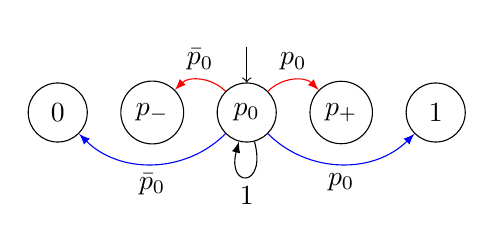
\begin{tikzpicture}
    \node[draw, minimum width=0.75cm, node distance=1.2cm, circle, initial above,initial text={} ] (bi) {$p_0$};
    \node[draw, minimum width=0.75cm, node distance=1.2cm, circle, left of=bi] (bm) {$p_-$};
    \node[draw, minimum width=0.75cm, node distance=1.2cm, circle, right of=bi] (bp) {$p_+$};
    \node[draw, minimum width=0.75cm, node distance=1.2cm, circle, right of=bp] (b1) {$1$};
    \node[draw, minimum width=0.75cm, node distance=1.2cm, circle, left of=bm] (b0) {$0$};

    \draw[-latex, red] (bi) to[out=45, in=135] node[black, above] {$p_0$} (bp);
    \draw[-latex, red] (bi) to[out=135, in=45] node[black, above] {$\bar p_0$} (bm);
    % \draw[-latex, red] (bi) to[out=45, in=135] node[black, above] {$q p_0$} (b1);
    % \draw[-latex, red] (bi) to[out=135, in=45] node[black, above] {$q \bar p_0$} (b0);
    \draw[-latex, blue] (bi) to[out=-45, in=-135]  node[black, below] {$p_0$} (b1);
    \draw[-latex, blue] (bi) to[out=-135, in=-45]  node[black, below] {$\bar p_0$} (b0);
    \draw[-latex, black] (bi) to[loop below] node[below, black] {1} (bi);
  \end{tikzpicture}
  \end{center}
  \caption{Illustration of the environment belief model for a single region, only transitions from the initial state $p_0$ are shown. Bars denote the complementary probability, i.e. $\bar p = 1-p$. When a high-quality measurement is received (blue edges), the belief transitions to $1$ with probability $p_0$ and to $0$ with probability $1-p_0$, whereas a low-quality measurement yields  beliefs $p_-$ or $p_+$. When no measurement is taken (black) the state does not change.}
  \label{fig:envmdp}
\end{figure}

We assume that regions of interest have been extracted from low-resolution satellite imagery, along with prior probability estimates for the likelihood that the regions exhibit certain traits. Here we restrict attention to \emph{risk regions} that may contain obstacles the rover can not traverse, and \emph{target regions} that are likely places where scientific samples can be extracted. We associate to each region $i$ a belief MDP $\MDP_{e_i}$ with five states $\zeta \in \{ 0, p_-, p_0, p_+, 1\}$ and three inputs $v \in \{ N, W, S \}$ for (N)o measurement, (W)eak measurement, and (S)trong measurement. The transition matrices are $T_N = I_5$,
\begin{equation}
  T_{S} = \left[\begin{smallmatrix}
    1        &  0  &  0  &  0  &  0   \\
    \bar p_- &  0  &  0  &  0  &  p_- \\
    \bar p_0 &  0  &  0  &  0  &  p_0 \\
    \bar p_+ &  0  &  0  &  0  &  p_+ \\
    0        &  0  &  0  &  0  &  1
  \end{smallmatrix}\right],
  T_{W} = \left[\begin{smallmatrix}
    1        &  0                &  0  &  0           &  0   \\
    0        &  1                &  0  &  0           &  0 \\
    0        &  \bar p_0         &  0  & p_0          &  0\\
    0        &  0                &  0  &  1           &  0 \\
    0        &  0  &  0  &  0  &  1
  \end{smallmatrix}\right].
\end{equation}
The outgoing transitions from $p_0$ are illustrated in Figure \ref{fig:envmdp}.

Given belief MDPs $\MDP_{e_i}$ for every region of interest, we construct the environment model $M_{env}$ as the parallel product
\begin{equation}
  \MDP_{env} = \MDP_{e_1} \otimes_{par} \MDP_{e_1}  \otimes_{par} \ldots \otimes_{par} \MDP_{e_n}.
\end{equation}

\paragraph{Specification}

The objective of the mission is to satisfy a scLTL specification $\varphi$ over propositions over states in $\MDP_{rov}$ and $\MDP_{env}$. Examples of such propositions include
\begin{itemize}
  \item Don't enter a risk region $R_1$ that may contain an obstacle: $\xi_r \not  \in R_1 \lor \zeta_1 = 0$.
  \item Collect a sample at region $R_2$: $\xi_r \in R_2 \land \zeta_2 = 1$.
\end{itemize}

We posit that the rover has a time window of length $T_r$ to fulfill its mission, and that the copter has battery sufficient to operate for a time $T_c$. In addition, the copter must land in a pre-designated landing area $X_l$ at the end of the execution. This auxiliary objective is straightforward to incorporate into \eqref{eq:coptervalue} by restricting the value iteration to policies that land safely with some high probability $1-\delta_l$.

\paragraph{Measurement model}

\begin{figure}
\begin{center}
    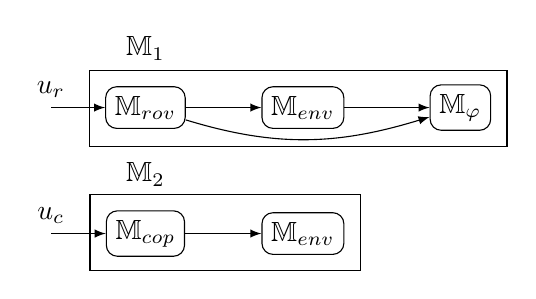
\begin{tikzpicture}
    \node[draw, node distance=2cm, rounded corners] (rover) {$\MDP_{rov}$};
    \node[draw, node distance=2cm, rounded corners, right of=rover] (environment) {$\MDP_{env}$};
    \node[draw, node distance=2cm, rounded corners, right of=environment] (fsa) {$\MDP_\varphi$};

    \draw[-latex] (rover) --  (environment);
    \draw[-latex] (environment) --  (fsa);
    \draw[-latex] (rover) to[out=-17, in=197] (fsa);

    \draw ([xshift=-2mm, yshift=2mm]$(rover.north west)$) rectangle ([xshift=2mm, yshift=-2mm]$(fsa.south east)$) {};
    \node[above of=rover, node distance=0.75cm] {$\MDP_1$};

    \draw[latex-] (rover) -- ++(-1.2,0) node[coordinate] (west) {} node[above] {$u_r$};

    \node[below of=rover, draw, node distance=1.6cm, rounded corners] (copter) {$\MDP_{cop}$};
    \node[draw, node distance=2cm, rounded corners, right of=copter] (env2) {$\MDP_{env}$};

    \draw[-latex] (copter) --  (env2);

    \draw ([xshift=-2mm, yshift=2mm]$(copter.north west)$) rectangle ([xshift=2mm, yshift=-2mm]$(env2.south east)$) {};
    \node[above of=copter, node distance=0.75cm] {$\MDP_2$};

    \draw[latex-] (copter) -- ++(-1.2,0) node[coordinate] (west) {} node[above] {$u_c$};

  \end{tikzpicture}
\end{center}
  \caption{Illustration of aggregate systems $\MDP_1$ and $\MDP_2$ constructed as serial products, where $\MDP_{env}$ is itself a parallel product.}
  \label{fig:agg}
\end{figure}


We connect the systems in serial as illustrated in Fig \ref{fig:agg}. The serial products are defined via connections that map the state of one system to the input of the next. These connections are defined as follows:
\begin{itemize}
  \item If the rover is adjacent to a region $R_i$ it takes a (S)trong measurement of that region,
  \item If the copter is at low altitude and in region $R_i$, it takes a (S)trong measurement of that region,
  \item If the copter is at high altitude and within distance $2$ of region $R_i$, it takes a (W)eak measurement of that region,
  \item The connection $C_\varphi$ defining the $\MDP_{rov} \otimes_{ser}^{C_\varphi} \MDP_{env}$ product is given by the truth value of atomic propositions for the state $(\xi_r, \xi_e)$.
\end{itemize}


\subsection{Illustrations}

We demonstrate the features of the proposed solution in a few example scenarios.

\paragraph{Scenario 1} Fig. \ref{fig:workspacemars} illustrates the Kimberly region in Mars Gale Crater where regions have been labeled as obstacles (red), risk regions (orange) and science target regions (blue). While the obstacle regions have been determined to be in-traversable, there is a sandy area $R_5$ and a rocky area $R_4$ that may be possible to cross. The objective is to collect a sample from any one of the three target regions while avoiding obstacles, i.e. the specification is
\begin{equation}
  \lnot \texttt{obstacle} \; \mathcal U \; \texttt{sA},
\end{equation}
where the atomic proposition $\texttt{obstacle}$ is $\True$ if the rover is in a risk region that contains an obstacle, and $\texttt{sA}$ is $\True$ if the rover is in a target region that contains a science sample.

A good way to use our method is as a way to determine when additional exploration is warranted. To illustrate we consider a scenario where the initial probability of specification satisfaction is high: there is a high estimated probability that a sample can be extracted from the easy-to-access region $A_3$. However, when the rover reaches $A_3$ it turns out to be empty and the mission is now associated with more risk. This motivates an exploration phase with the hope that the uncertainty can be reduced. In Fig. \ref{fig:marstrajectories} the team behavior is illustrated for two configurations of the environment: one where the specification can be satisfied and one where it is infeasible.

\begin{figure}
  \begin{center}
    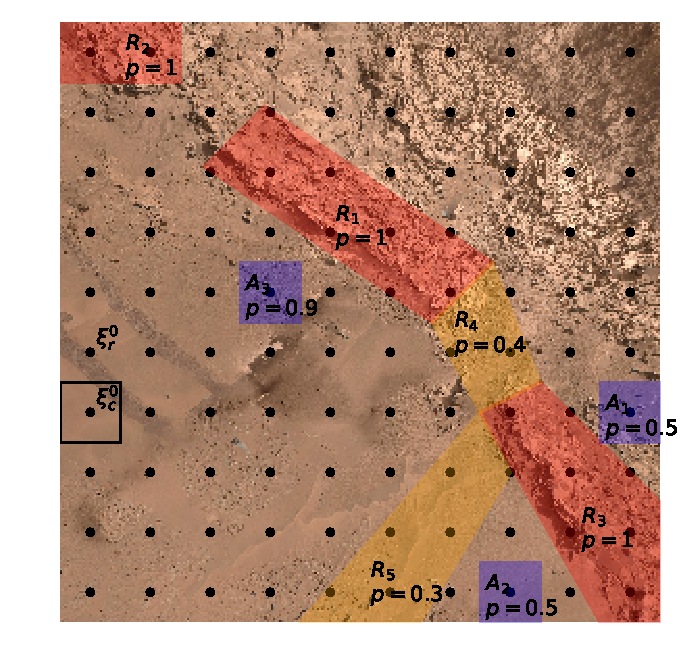
\includegraphics[width=0.6\columnwidth]{2figs/arena-MARS.pdf}
  \end{center}
  \caption{2D view of the work space where regions of interest $R_i$, $A_i$ are marked along with associated prior probabilities. Each abstract state is illustrated with a dot. The black square marks the required landing zone for the copter.}
  \label{fig:workspacemars}
\end{figure}

\begin{figure}
\begin{center}
  \footnotesize
  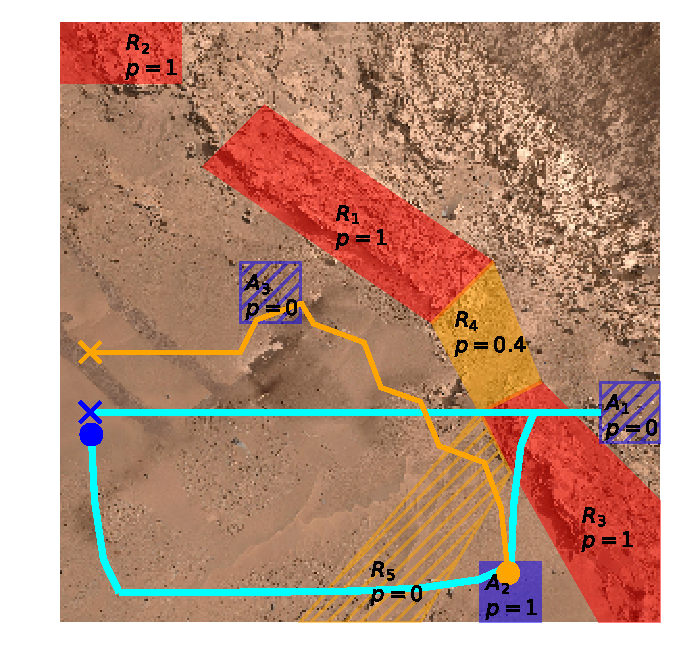
\includegraphics[width=0.45\columnwidth]{2figs/trajectory0.pdf} ~ 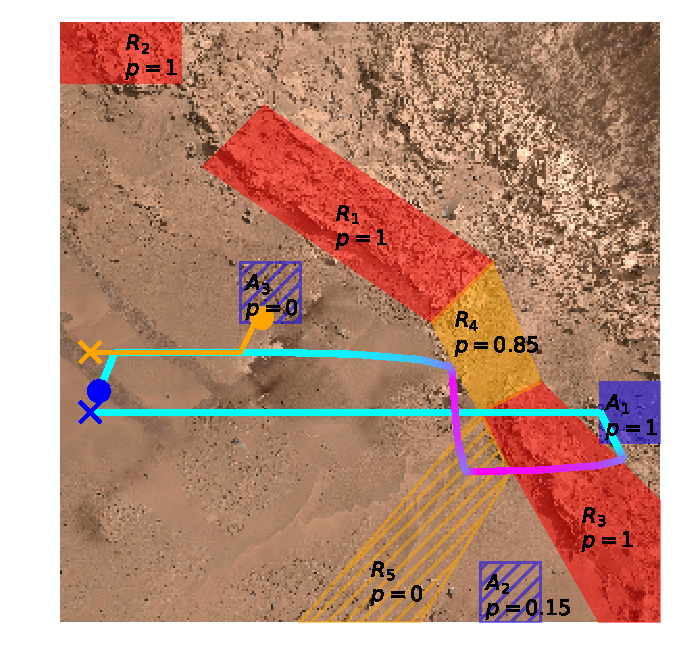
\includegraphics[width=0.45\columnwidth]{2figs/trajectory1.pdf}
  \begin{tikzpicture}
    \begin{axis}[width=0.5\columnwidth,
                  height=0.3\columnwidth,
                  xlabel={$t$},
                  ylabel={$\mathbf{P}(\varphi)$},
                  ymin = 0,
                  ymax = 1,
                  xticklabels = none,
                  xtick = {},
                  axis y line=middle,
                  axis x line=middle,
                  every axis x label/.style={
                      at={(ticklabel* cs:1.05)}
                  },
                  every axis y label/.style={
                      at={(0.,1.05)},
                  anchor=south,
                  }
                  ]
      \addplot[mark=none, blue] table[x index=1, y index=0] {2figs/proba0.txt};
      \draw[draw=none, fill = mission, opacity = 0.3] (axis cs:0,0) rectangle (axis cs: 35,1);
      \draw[draw=none, fill = explore, opacity = 0.3] (axis cs:35,0) rectangle (axis cs: 251,1);
      \draw[draw=none, fill = mission, opacity = 0.3] (axis cs:251,0) rectangle (axis cs: 321,1);
    \end{axis}
  \end{tikzpicture} ~
  \begin{tikzpicture}
    \begin{axis}[width=0.5\columnwidth,
                  height=0.3\columnwidth,
                  xlabel={$t$},
                  ylabel={$\mathbf{P}(\varphi)$},
                  ymin = 0,
                  ymax = 1,
                  xticklabels = none,
                  xtick = {},
                  axis y line=middle,
                  axis x line=middle,
                  every axis x label/.style={
                      at={(ticklabel* cs:1.05)}
                  },
                  every axis y label/.style={
                      at={(0.,1.05)},
                  anchor=south,
                  }
                  ]
      \addplot[mark=none, blue] table[x index=1, y index=0] {2figs/proba1.txt};
      \draw[draw=none, fill = mission, opacity = 0.3] (axis cs:0,0) rectangle (axis cs: 35,1);
      \draw[draw=none, fill = explore, opacity = 0.3] (axis cs:35,0) rectangle (axis cs: 248,1);
      % \draw[draw=none, fill = mission, opacity = 0.3] (axis cs:251,0) rectangle (axis cs: 321,1);
    \end{axis}
  \end{tikzpicture}
\end{center}
  \caption{Trajectories of the rover (orange) and copter (teal/purple for low/high elevation), and associated probabilities of specification satisfaction, for two environment configurations. In the initial mission phase (green), the rover moves towards a target area with a high sample probability of 0.9. However, the target area unexpectedly turns out to not contain a sample and the probability of specification satisfaction decreases to around 0.5. This triggers an exploration phase (blue) where the copter attempts to find out whether the mission can be completed or not. This succeeds in the illustration to the left and the rover proceeds with its mission, but fails in the case to the right and the mission is aborted.}
  \label{fig:marstrajectories}
\end{figure}


\paragraph{Scenario 2} To further illustrate intelligent behavior we consider an artificial example depicted in Fig. \ref{fig:workspace1}. The specification is as follows: either collect samples of types $A$ and $B$, or collect a sample of type $C$, while avoiding obstacles. Letting $\lozenge_o \varphi = \lnot \texttt{obstacle} \; \mathcal U \; \varphi$, the specification can be written
\begin{equation*}
  \left( \lozenge_o \texttt{sA} \land \lozenge_o \texttt{sB} \right)  \lor \left( \lozenge_o  \texttt{sC}  \right).
\end{equation*}
The atomic proposition \texttt{sA} is $\True$ if $\xi_r \in A$ (rover is in region $A$) and $\zeta_A = 1$ (sample detected in $A$), and similarly for \texttt{sB} and \texttt{sC}. We assume that the rover can move for $T_r = 15$ time steps, and that the copter has enough battery to move for $T_c - T_r = 30$ time steps (including changes of altitude). With the two-stage approach described in Section \ref{sec:stochopt} we can then compute 1) a value function $V_r(\xi_r, \xi_e, \xi_\varphi)$ and corresponding policy for the rover, and 2) a policy for the quadrotor that maximizes the probability of reaching a state where $V_r(\xi_r^0, \xi_e, \xi_\varphi^0)$ is either close to 0 or close to 1.

Executions generated from the resulting copter and rover policies are shown in Fig. \ref{fig:copter_executions} for different configurations of the true environment state. With only prior knowledge about the environment, the probability that the rover can satisfy the specification is $V_r(\xi_r^0, \xi_e^0, \xi_\varphi^0) = 0.25$. However, after the copter exploration all uncertainty is removed: for the two upper examples in Figure. \ref{fig:copter_executions}, $V_r(\xi_r^0, \xi_e^{T_{c}}, \xi_\varphi^0) = 1$ where $\xi_e^{T_c}$ is the environment belief state after copter exploration, and for the lower examples $V_r(\xi_r^0, \xi_e^{T_{c}}, \xi_\varphi^0) = 0$. This shows that the generated policy explores the environment in a way that efficiently reduces uncertainty about whether the specification can be satisfied.

\begin{figure}
  \begin{center}
    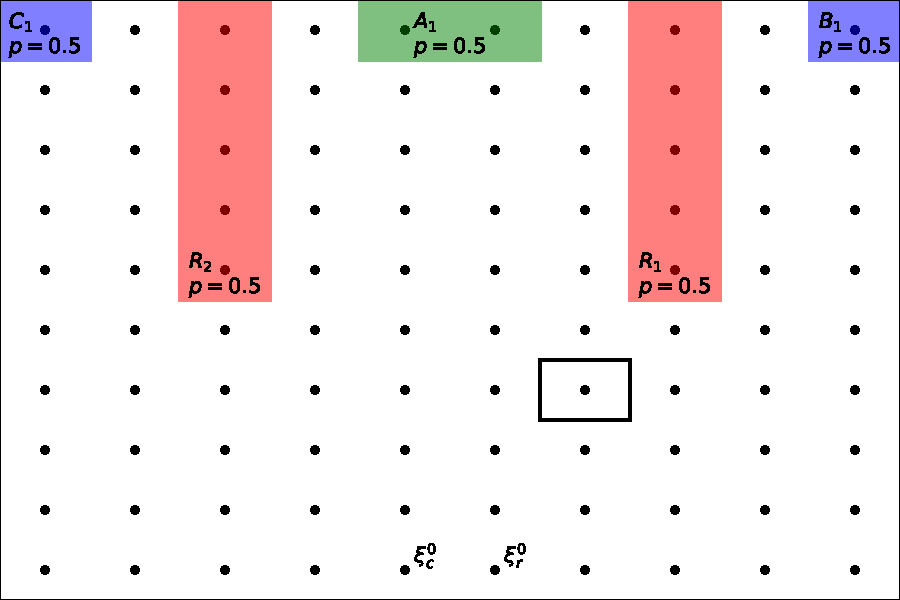
\includegraphics[width=0.6\columnwidth]{2figs/arena.pdf}
  \end{center}
  \caption{2D view of the work space where regions of interest $R_1$, $R_2$, $A$, $B$, and $C$ are marked along with associated prior probabilities. Each abstract state is illustrated with a dot. The black square marks the required landing zone for the copter.}
  \label{fig:workspace1}
\end{figure}

\todo[inline]{Connect this example with the Terraswarm example of Sheshia.}

\begin{figure}
	\begin{center}
	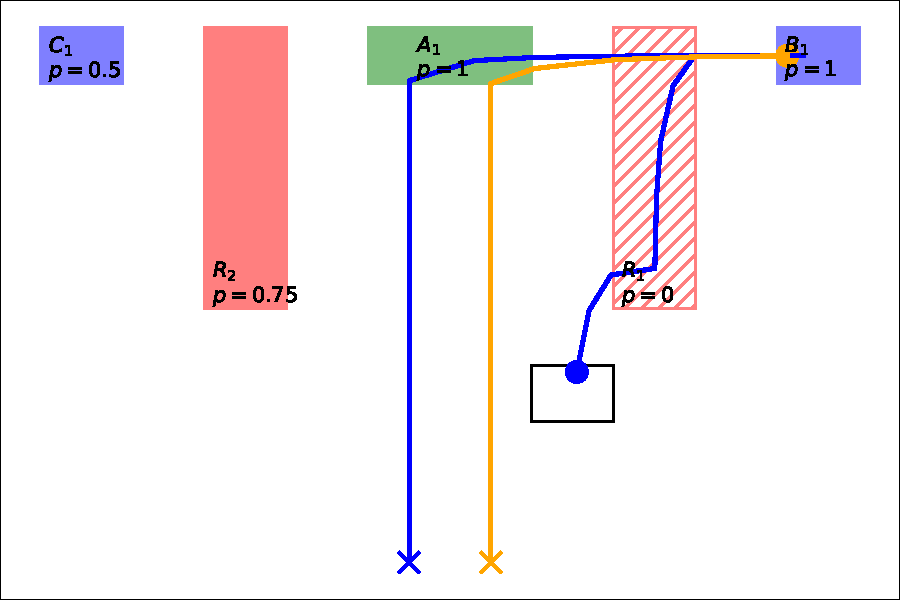
\includegraphics[width=0.4\columnwidth]{2figs/exp0-map.pdf} ~
	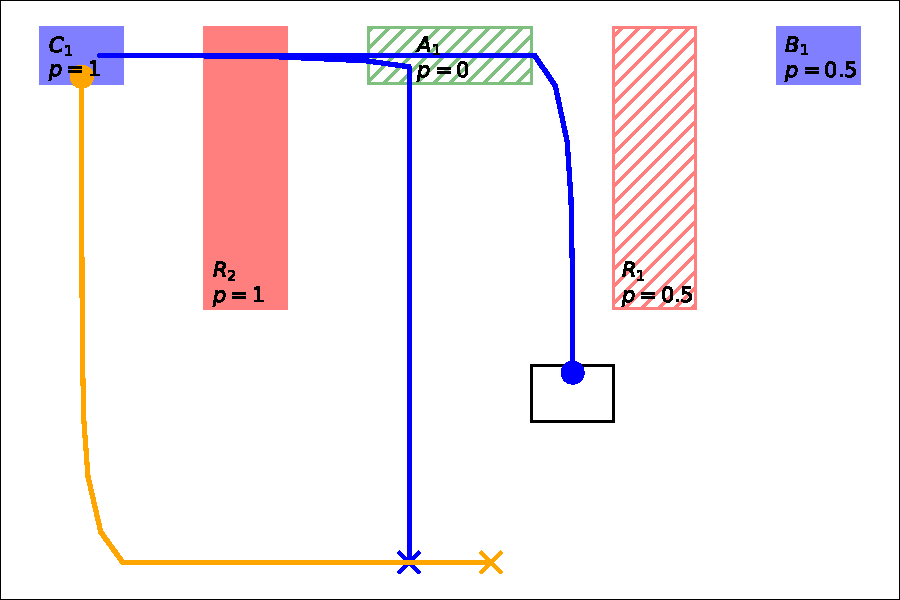
\includegraphics[width=0.4\columnwidth]{2figs/exp1-map.pdf} \\
	\vspace{1mm}
	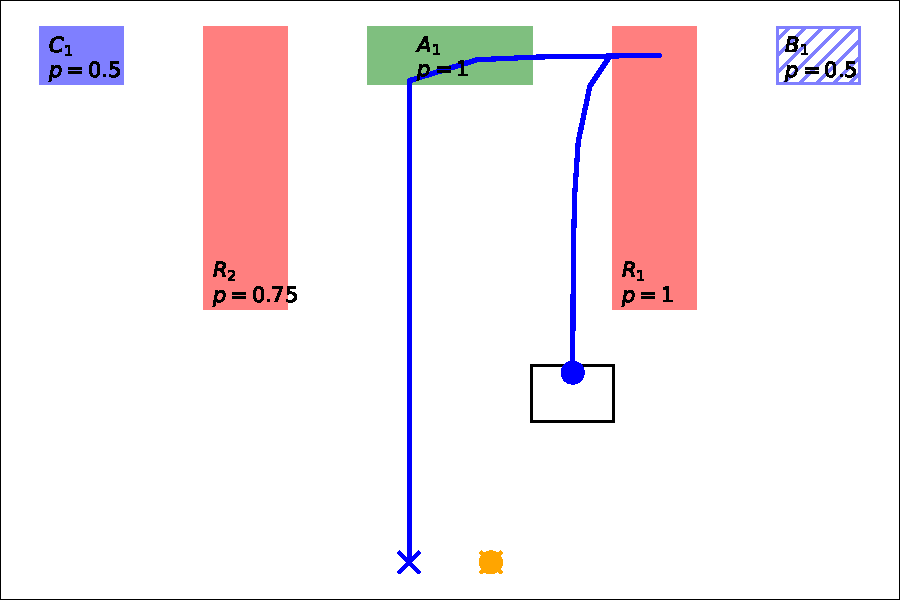
\includegraphics[width=0.4\columnwidth]{2figs/exp2-map.pdf} ~
	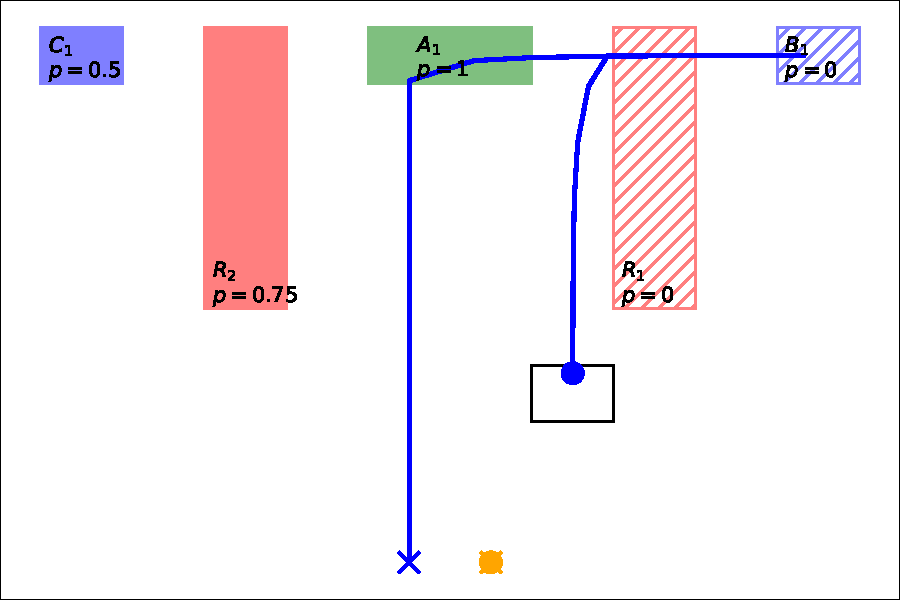
\includegraphics[width=0.4\columnwidth]{2figs/exp3-map.pdf}
	\end{center}
	\caption{Illustration of the copter and rover policies for different environment configurations: a shaded region indicates that the true state is equal to 0 (i.e. no sample or obstacle). The region probabilities indicate the belief states after the copter exploration phase. Copter trajectories are shown in blue, and rover trajectories in orange, if the specification can not be satisfied the rover does not move. All four executions are generated by the exact same policies; they adapt according to measurements received during the execution.}
	\label{fig:copter_executions}
\end{figure}

% \begin{figure}
%   \begin{center}
%     \footnotesize
%     \begin{tikzpicture}
%       \node[inner sep=0] (p1) {
\includegraphics[height=0.24\columnwidth]{2figs/value-rov.pdf}};
%       \node[inner sep=0, anchor=west] at ([xshift=2mm]$(p1.east)$) (p2) {
\includegraphics[height=0.24\columnwidth]{2figs/value-cop.pdf}};
%       \node[inner sep=0, anchor=west] at ([xshift=2mm]$(p2.east)$) (n1) {
\includegraphics[height=0.24\columnwidth]{2figs/cbar.pdf}};
%       \node at ([yshift=2mm]$(p1.north)$) {$V_0^1(\xi_r, \xi_e^0, \xi_\varphi^0)$};
%       \node at ([yshift=2mm]$(p2.north)$) {$V_0^2(\xi_c, \xi_e^0)$};
%       \node at ([xshift=6mm]$(n1.north east)$) {$p = 0.48$};
%       \node at ([xshift=6mm]$(n1.south east)$) {$p = 0$};
%     \end{tikzpicture}
%   \end{center}
%   \caption{Illustration of value functions. As can be seen, the advantage of the copter is equivalent to having the rover's initial state be near a target region.}
%   \label{fig:values1}
% \end{figure}


\section{Conclusion}
\label{sec:conclusion}

We presented a modeling framework for multi-agent systems operating in uncertain environments, and proposed a dynamic programming-based solution to the problem of in a specification-guided fashion determining what areas of the environment to explore. The solution method works with arbitrary MDPs, so there is significant flexibility in modeling which can be done via formal abstractions, sampling-based methods, etc. As demonstrated, value iteration is possible without constructing the aggregate systems explicitly, but scalability remains an issue since the representation of the value function grows linearly with the size of the aggregate state space (which grows exponentially with the number of system components). As discussed in Section \ref{sub:factored_mdp_work}, it can not be expected that sparse representations exist for the true value function, but sparse value function representations can potentially yield approximate methods that improve scalability further. This is one direction for future research. Another way to partially circumvent scalability issues is to iteratively refine the models in a specification- and exploration-guided fashion, as explored e.g. in \cite{Nilsson2017}. For instance, exploration may reveal that certain regions of interest should be treated as multiple regions, but at this point more information is known which reduces the size of the overall belief space. Thus, iterative exploration and model refinement can limit the number of uncertain region labels over time.  


\bibliographystyle{abbrvnat}
\bibliography{2_references,AliAgha3}

% AliAgha,references_combined, AliAgha3
\end{document}
